\documentclass{scu-thesis}
\usepackage{amsmath}	% for advanced typesetting of mathematics
\usepackage{graphicx}	% for including graphics
\usepackage{natbib}	% for better citation styles
\usepackage{txfonts}	% for using the Times-Roman font
\usepackage{blindtext}

% These must be set first ... the rest of the thesis commands rely on them.

\author{Shannen Edwin}
\author{Dominic Magdaluyo}
\title{Doorbell for the Hearing Impaired}
\department{Department of Computer Engineering}
\degree{Bachelor of Science in Computer Science \& Engineering}


% Only bachelor's theses should have multiple authors and/or be from
% multiple departments.  Signatures required:
%
% Bachelor's theses: advisor(s), department chair(s)
% Master's theses: advisor, reader, department chair
% Doctoral theses: doctoral committee (including advisor), department chair

\begin{document}
\frontmatter
\signature{Thesis Advisor}
\signature{Department Chair}


\maketitle
\begin{abstract}
A good abstract is a concise summary (1--2 paragraphs) of the entire
project: introduction, problem statement, work accomplished, results,
conclusions, and recommendations. When you write the abstract, imagine
that the reader will not read anything else, but that you must get
your major point across immediately. This requires efficiency of words
and phrases. An abstract is written to stand alone, without jargon or
reference to figures and tables in the report body.
\end{abstract}


\tableofcontents
\listoffigures
\listoftables

\mainmatter
\chapter{Introduction}

\section{Problem and Motivation}

Doorbells and knocking are often useless for those that are audibly impaired. Someone with hearing impairments needs to depend on other residents to answer the door for them or purchase expensive equipment to send them phone notifications. Depending on the neighborhood, the ability to know there’s a visitor at the door is essential for quality of life including community involvement and package delivery.

The inspiration for this system came from one of our homes. Since the doorbell stopped functioning within certain parts of the home, it was easy to see the impact not knowing someone is at the door can have on a resident due to the inability to hear a doorbell. This also created a burden on others within the house due to repeated doorbell presses and searching for person the visitor intends to speak with. 

\section{Solution}
In this section, we look at current solutions that exist and provide insight into our solution.

\subsection{Current Solutions}
Current solutions are limited in supporting these individuals. Louder doorbells are useless to those that are completely deaf and can be bothersome for housemates that are not hearing impaired. Some solutions like Physen’s Doorbell Kits are viable and affordable solutions but they are not scalable. Physen and other manufacturers make closed systems that offer limited options. There are also doorbells such as the Ring’s doorbell which can send a notification to a phone; however, this solution can be expensive. Ring’s security camera doorbell costs \$100. That can be well above the financial capabilities of many people. Especially among deaf individuals, we find that unemployment is high at 47\% \cite{pdf:deaf-employment} and many in this population are senior citizens; therefore, finding an affordable solution is very important. There are also scalable options such as the IFTTT platform, which can connect various IoT devices that are readily available on their platform. Unfortunately, this system is closed. Companies must be registered to their system and developed for it. The IFTTT platform also drops and adds devices to the system without warning. The devices available to help hearing impaired individuals in the IFTTT platform can be expensive such as connecting the Ring doorbell to Philips Hue lights which can add up to at least \$200.

%Older version of this section
%Current solutions are limited in supporting these individuals. Louder doorbells are useless to those that are completely deaf and can be annoying for housemates that are not hearing impaired. Current light systems are not integrated into the house and must be carried around the house (or multiple installments are needed, thereby increasing the cost). Furthermore, the light systems may be easily missed if not facing the device or if in a well-lit room. Video doorbells are expensive and require a smartphone to interface with it. The notifications may be missed during the time frame where a person is at the door. A useful alternative is smart wearables but those are limited in battery life. For example, the Apple Watch Series 4 is advertised to last 18 hours on average use \cite{website:apple-watch-battery} which is not useful for a person when sleeping. Designing a low-cost solution was important to the team, as unemployment among deaf individuals is high at 47\% \cite{pdf:deaf-employment}. Generally, hard of hearing individuals are senior citizens who do not have much money. A simple and affordable solution would improve their lives greatly. The hearing impaired community already struggle enough and providing an affordable option to doorbells is essential in keeping them aware of their surroundings and being part of their communities.

\subsection{Contribution}
Our solution is a proof of concept for a scalable and affordable system. Our doorbell is low power and connects to a modular system. A gateway consisting of a Raspberry Pi Zero W and an XBee will be able to connect any device a user desires by using Node-RED.
%To tackle these issues, our solution would aim at integrating a system into the entire household by using Philips Hue light fixtures or, as a cheaper alternative, providing LED strips, removing the need for a portable device that may be easily forgotten. Furthermore, the system will give the user options on a configuration that works best for their home. On top of that we will provide a low power vibration bracelet solution. This would be sleek so that it can be worn while sleeping while providing a gentle but noticeable vibration. The bracelet could be charged while away from the house, so a user will always be able to use it once in the house. Together, our system will be low cost while providing more functionality towards the hearing impaired.

\chapter{Requirements}

\section{Description}
In this chapter, we list the functional and nonfunctional requirements prioritizing them from top to bottom. In section 2.2, we list functional requirements by critical, recommended, and suggested and these describe what the system will do. In section 2.3, we list non-functional requirements in the same way and these describe how the system will perform. Lastly, in section 2.4, we discuss our design constraint and how it affects the scope of this project.

\section{Functional Requirements}
\begin{itemize} 
\item Critical
	\begin{itemize} 
	\item Doorbell will activate light system
	\end{itemize}
\item Recommended
	\begin{itemize} 
	\item Doorbell will activate vibration system
	\item Doorbell is integratabtle with other light/vibration devices available
	\item The System will be low power
	\end{itemize}
\item Suggested
	\begin{itemize} 
	\item Doorbell will not communicate over WiFi
	\end{itemize}
\end{itemize}
\section{Non-Functional Requirements}
\begin{itemize} 
\item Critical
	\begin{itemize} 
	\item The system will be cheap, ideally \$50 or less for a full house integration
	\end{itemize}
\item Recommended
	\begin{itemize} 
	\item The system will be able to connect to various types of devices to allow preferred devices per user
	\end{itemize}
\item Suggested
	\begin{itemize} 
	\item The system has an appealing aesthetic
	\end{itemize}
\end{itemize}
\section{Constraints}
The constraint of our design is that we are not building from the ground up. This makes achieving our goal of an affordable system very difficult as we will be using already built parts. As such is the case, we will have to design this system as a proof of concept.
\chapter{Use Case Diagram}

\section{Description}
The use case diagram (Figure \ref{fig:usecase}) shows the potential functions of our system for two actors: the Resident and the Visitor. Our use cases are listed in the following section by which actor is allowed the action and what preconditions, postconditions, and/or exceptions are there for the specific use case in our system.

\begin{figure}[h]
  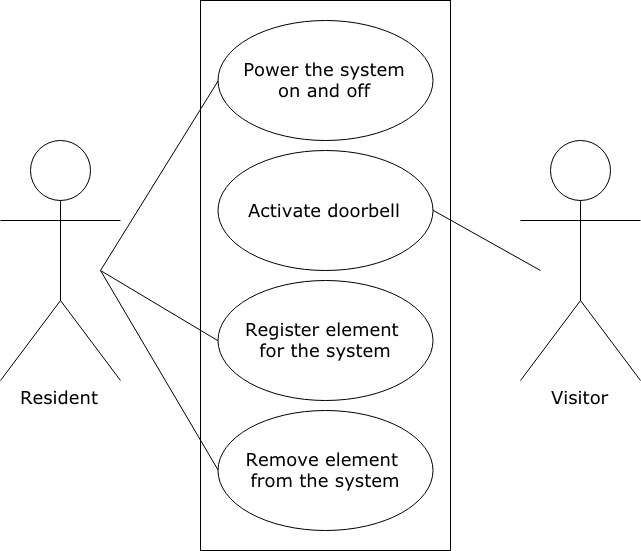
\includegraphics[width=0.8\textwidth]{UseCase.png}
  \centering
  \caption{Use Case Diagram}
  \label{fig:usecase}
\end{figure}

\section{Functionality}

\subsection{Power System On and Off}
\begin{description}
\item [Actor:] Resident
\item [Goal:] Setting up system and personalizing it
\item [Postcondition:] System should safely shut off or turn on with previous settings
\end{description}
\subsection{Activate Doorbell}
\begin{description}
\item [Actor:] Visitor
\item [Goal]: Alert the Resident, that someone is at the door
\item [Precondition:] System is successfully activated with a device paired to it
\item [Postcondition:] Alert the Resident through their connected device(s)
\item [Exceptions:] Nothing happens if System is not active or device is disconnected
\end{description}
\subsection{Register Element to the System}
\begin{description}
\item [Actor:] Resident
\item [Goal:] Connect a device so Resident may be alerted of Visitor at door
\item [Precondition:]System is powered on successfully
\item [Postcondition:] Device is registered successfully to system and will be activated once prompted
\item [Exception:] Unsuccessful device registration and prompt user of error in pairing
\end{description}
\subsection{Remove Element from the System}
\begin{description}
\item [Actor:] Resident
\item [Goal:] Unregister device from the system when no longer using it
\item [Precondition:] System should be on
\item [Postcondition:] Device successfully unregistered
\end{description}
\chapter{Activity Diagrams}

\section{Description}
The activity diagrams show the potential paths of actions a user may take with the system. For the Resident actor (Figure \ref{fig:residentdiagram}), upon turning on a system, the user may register or remove devices. The system will be then available and a user may receive a response when the doorbell is pressed. From any of these actions a user may take, they may also power the system off. For the Visitor actor (Figure \ref{fig:visitordiagram}), when the system is on, the user will be able to activate the doorbell by a button and have one of the connected devices respond to the Resident actor.

\begin{figure}[ht]
  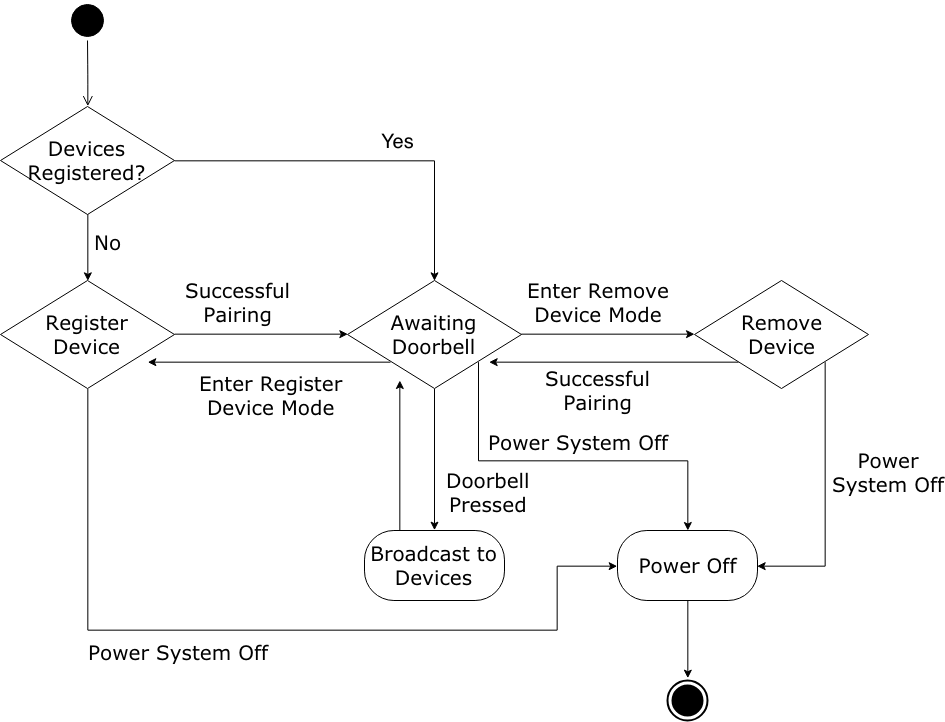
\includegraphics[width=0.8\textwidth]{ResidentActivityDiagram.png}
  \centering
  \caption{Resident Activity Diagram}
  \label{fig:residentdiagram}
\end{figure}

\begin{figure}[ht]
  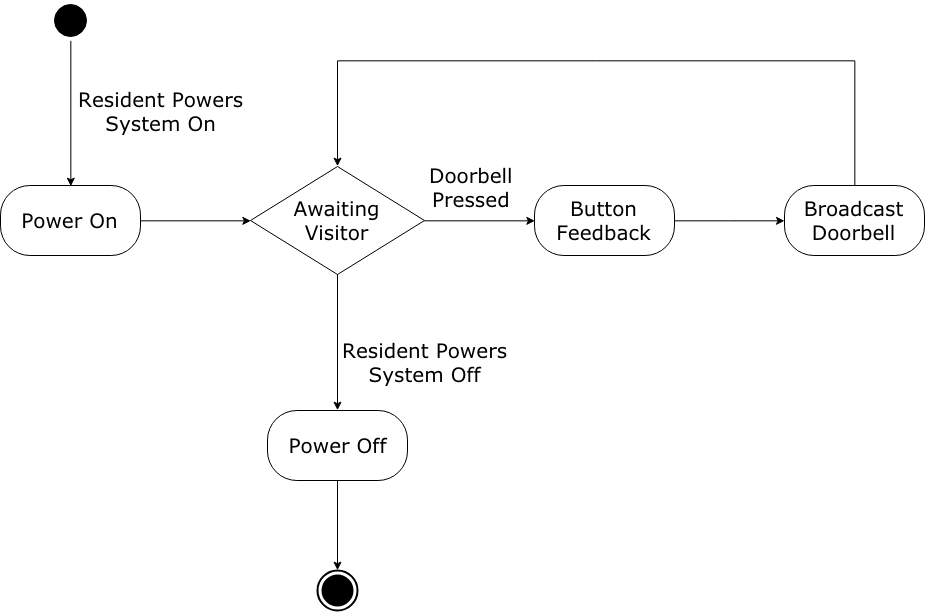
\includegraphics[width=0.8\textwidth]{VisitorActivityDiagram.png}
  \centering
  \caption{Visitor Activity Diagram}
  \label{fig:visitordiagram}
\end{figure}
\chapter{Architecture Diagram and Conceptual Model}

\section{Architecture}
The system relies on an event-based architecture. As shown in the architecture diagram (Figure \ref{fig:architecture}), the arrows show the flow of data between the different components of the system. The doorbell button triggers an event that goes to the Raspberry Pi Zero which acts as an announcer in this architecture. This event tells the announcer to broadcast the appropriate doorbell event to all types of devices currently registered in the system. The doorbell offers feedback to the Visitor in the form of a pulsating light to confirm that the button was pressed and the event was broadcast to the Resident's devices. The arrow going to the Raspberry Pi Zero from the Home Network is to confirm that the devices received the broadcast event.

\begin{figure}[ht]
  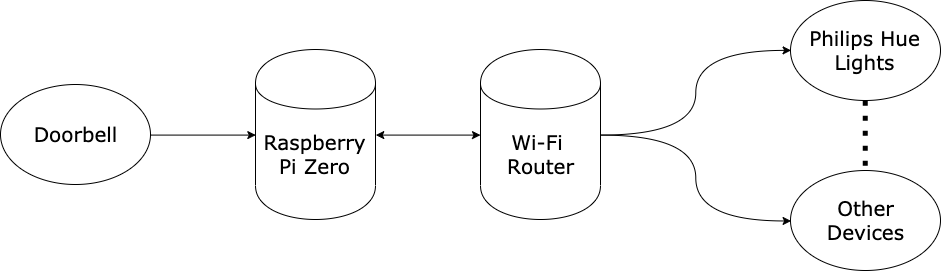
\includegraphics[width=0.9\textwidth]{Architecture-updated.png}
  \centering
  \caption{Architecture Diagram}
  \label{fig:architecture}
\end{figure}

\section{Conceptual Model}
The system uses the Raspberry Pi Zero as the main gateway. A router will be necessary in communicating to other devices in the household. The button of the doorbell will be attached to the an Arduino and communicate with the Raspberry Pi Zero.

\begin{figure}[ht]
  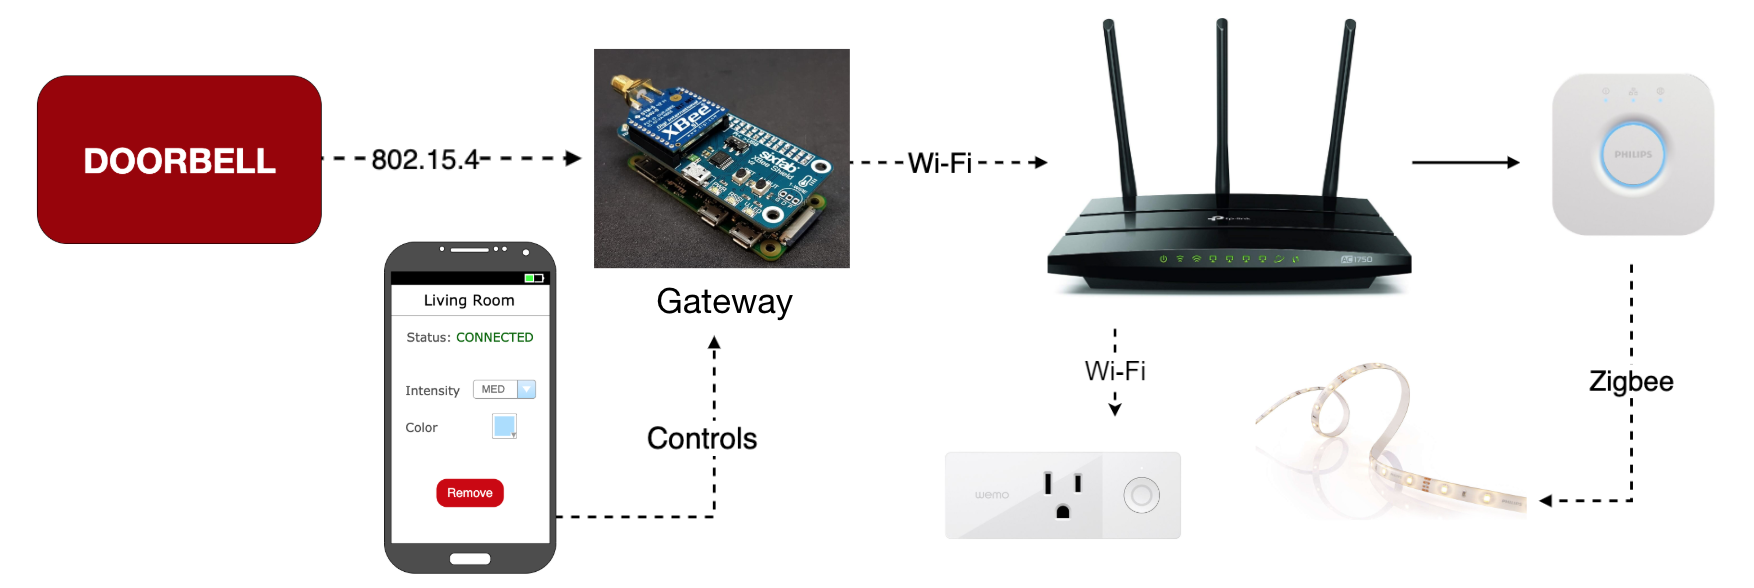
\includegraphics[width=0.8\textwidth]{senior-design-model.png}
  \centering
  \caption{Conceptual Model}
  \label{fig:conceptualmodel}
\end{figure}
\chapter{Technology Used and Design Rationale}

\section{Description}
In this chapter, we discuss the necessary devices and technology needed for this system and our reasoning for their choice in our design.

\section{Communication Protocols}
In the IoT world, there are a few communication protocols that we could use. In the following subsections, we go over the benefits and disadvantages of using each protocol.

\subsection{802.11 (Wi-Fi)}
802.11 is a common protocol with 802.11 access points present in many places today. It has high bandwidth at 11 Mbps and is supported by many devices. It is powerful and has moderate range between 30 and 100 meters. Unfortunately, this is a high power protocol which is not ideal for components in our system that will run on battery \cite{website:bluetooth-vs-wifi}.

    In our design, we decided to use this protocol in only broadcasting to devices connected to our system that will relay notifications to the user. Most likely these devices will have consistent power and will already be connected to the user’s WiFi network.

\subsection{802.15.1 (Bluetooth)}
802.15.1 is another common protocol. Many devices come with bluetooth to provide low range, moderate bandwidth connections. The bandwidth is moderate at 800 kbps while also providing moderate power consumption. The range is low at about 5 to 30 meters which is not useful if components of our system are placed far away from our central gateway. 

    In our design, we decided to use this protocol in broadcasting to devices connected to our system like 802.11 and for connecting a smartphone application to the gateway. The smartphone application would allow an average user to control the system as necessary for themselves.

\subsection{802.15.4 (Zigbee)}
802.15.4 is more commonly use in IoT applications. It is useful for it’s low power consumption and far range (about 100 meters). It has low bandwidth but that is not a problem for most IoT applications that may only require simple relays of information between devices. Most development uses Zigbee, a application layer protocol, that provides security and optimization for home automation.
 
    In our design, we decided to only go with 802.15.4. Development with Zigbee is covered under the Zigbee Alliance which would require us applying into the alliance. Considering the scope of this project, this seemed like an unnecessary delay. Furthermore, we don’t need the benefits of Zigbee to show a proof of concept. We found that 802.15.4 would be best in broadcasting between the doorbell and the gateway. This provides good range and allows the doorbell to consume less power than other communication protocols.

\section{Hardware}
Our system consists of edge devices and a gateway. The edge devices are the doorbell and the devices relaying notifications to the user. The gateway is made up of a Raspberry Pi Zero W and an XBee. The gateway will receive a notification from the doorbell and will notify the other devices through a home network.

\subsection{Gateway}
The gateway consists of a Raspberry Pi Zero W and an XBee. XBee is a programmable module from DigiKey. The S1 variant can use either 802.15.4 or Zigbee depending on the firmware flashed. Furthermore, it uses serial Tx and Rx to communicate so it can be added easily to any module. The Raspberry Pi Zero W was favorable to us as it would make our development easier being a familiar Unix-based system and having a vast open-source community. Furthermore, it is low cost and the W variant comes with Bluetooth and WiFi. Using these protocols, we can communicate to various devices connected to a home network through an access point.

\subsection{Doorbell}
The doorbell was originally intended to be Texas Instruments’ SensorTag C2650. The SensorTag has the option of either using Bluetooth or 802.15.4, which can be configured by flashing different firmware. SensorTag comes with many sensors which we thought would be great for us to experiment with such as the motion sensor. It was also advertised to last for two years using a lithium coin battery. This is a huge advantage as we don’t want users to be changing the battery often for the device.

    We eventually decided it was best to move away from SensorTag due to issues covered in a later chapter. Our solution became to use two XBees to communicate with each other. We knew that two XBees would work so long as they had the same parameters flashed. To accomplish this, we decided to use Arduino as the main processor for the doorbell. We used Arduino Uno for prototyping but Arduino Nano would be the best option in order to maintain a low power solution. Using an Arduino shield, interfacing with the XBee was simple using an XBee library from DigiKey.
    
    For the doorbell, we also wanted a visitor to have feedback that the doorbell was pressed. A common occurrence in pressing a doorbell is hearing the doorbell chime, informing the visitor that the doorbell is working and has sent a notification to the resident. We decided that an LED pulse would accomplish this same effect. Using an Illuminated Momentary Pushbutton from Adafruit, we were able to simply accomplish this in our doorbell.

\subsection{Conneced Devices}
A Philips Hue LED strip was used to test the implementation. Although expensive, Philips Hue has well-designed devices with an open API to make it easy to integrate into the system. Since this is just a proof of concept, showing the system working was a larger concern.

\section{Software Development}
Software consisted of C/C++, Python and Node-RED. The software was used in different ways in the system and is described in more detail in the following subsections.

\subsection{Doorbell Software}
The doorbell software is written in Arduino code which is based off of C/C++. The Arduino board can communicate to the XBee using the already available serial library. Since Arduino runs code continuously in a loop, the code waits for a trigger from the doorbell press. On press, the LED pulses to notify the visitor that the button is broadcasting. The XBee will send a broadcast. Any XBee with the same parameters in range will receive the packet.

\subsection{Gateway Software}
The gateway’s software comprised mostly of Node-RED. Created by IBM for IoT applications and written in Javascript, Node-RED uses flow programming to trigger nodes. Each node is a block that runs a process when triggered and provides an output that can trigger another node or end the flow. Using a ‘start-up-trigger’ node, the application will immediately start the flow when the Node-RED server starts. The flow will then wait to receive serial output from the XBee through the Pi’s Rx pin. When the node returns, the flow will split and notify all of the connected devices in the house each with their own respective nodes. To avoid unnecessary spawning of node processes and causing undefined behavior from doorbell spam, the flow waits for all nodes of notification devices to return. With the ‘wait-paths’ node, once all nodes return, the flow is repeated.

\subsection{Broadcasting Software}
With Raspberry Pi’s versatility as a Unix-based system, any programming language can be used to activate the connected devices. In our testing, the APIs were available in Python. With Node-RED, any script can be run using an ‘exec’ node. Furthermore, since Node-RED is open source, anyone can create nodes for use by creating a .json, .js, and .html file. Creating nodes are simple. With some technical knowledge, a growing network of nodes could be created for this application and may already be available for many devices.
\chapter{Conceptual Model}

\section{Description}
The system will use the Raspberry Pi Zero as the main computer. A router will be necessary in communicating to other devices in the household. The router can be performed by the Raspberry Pi Zero if necessary. The button of the doorbell will be attached to the Raspberry Pi Zero.

\begin{figure}[h]
  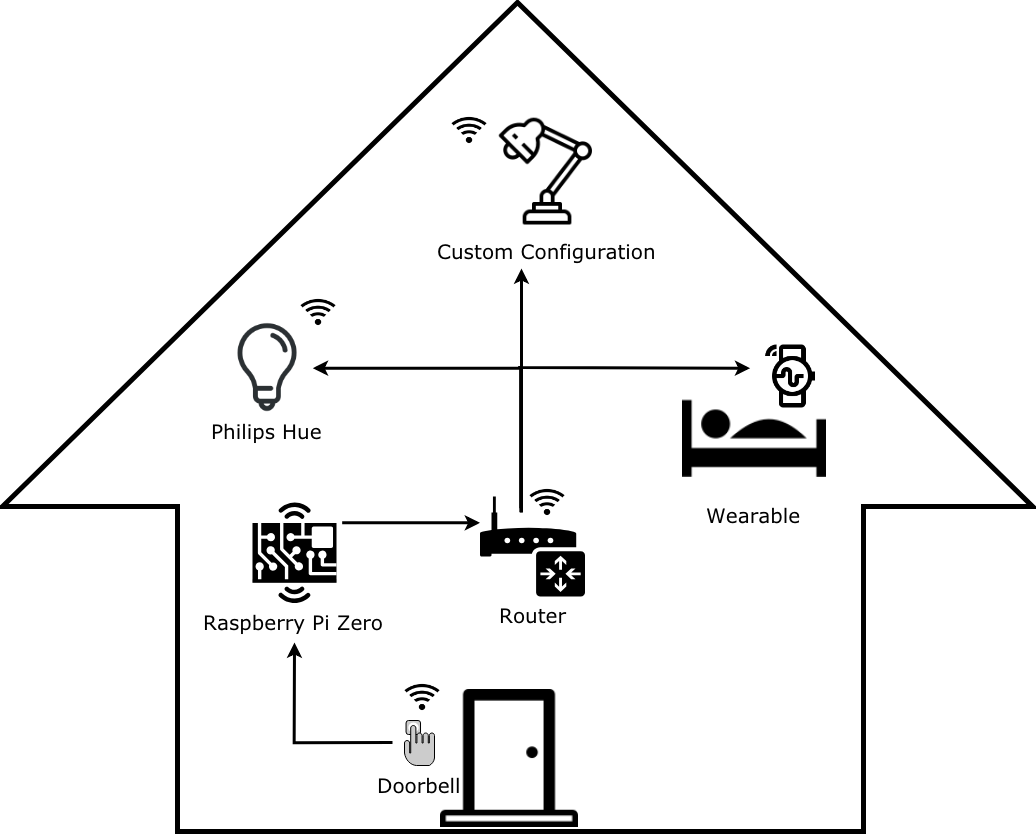
\includegraphics[width=0.8\textwidth]{ConceptualModel.png}
  \centering
  \caption{Conceptual Model}
  \label{fig:conceptualmodel}
\end{figure}
\chapter{Test Plan}

\section{Description}
\chapter{Risk Analysis}

%\section{Description}

\begin{table}[h!]
\begin{tabular}{|c|l|c|c|c|l|}
\hline
\begin{tabular}[c]{@{}c@{}}Risk\\ Name\end{tabular} & \multicolumn{1}{c|}{Consequences} & Probability & \begin{tabular}[c]{@{}c@{}}Severity\\ (0-10)\end{tabular} & Impact & \multicolumn{1}{c|}{\begin{tabular}[c]{@{}c@{}}Mitigation\\ Strategies\end{tabular}} \\ \hline
Time & Behind on deadlines. & 0,7 & 9 & 6.3 & Follow the development timeline. \\ \hline
\begin{tabular}[c]{@{}c@{}}Compatibility\\ Issues\end{tabular} & \begin{tabular}[c]{@{}l@{}}Will delay the development \\ of the system.\\ Spend unnecessary money.\end{tabular} & 0.6 & 7 & 4.2 & \begin{tabular}[c]{@{}l@{}}Research technologies and their \\ compatibility in full.\\ Discuss with advisor in \\ approaches to resolving issues.\end{tabular} \\ \hline
\begin{tabular}[c]{@{}c@{}}Network\\ Issues\end{tabular} & \begin{tabular}[c]{@{}l@{}}Will delay the development \\ of the system.\end{tabular} & 0.35 & 9 & 3.15 & \begin{tabular}[c]{@{}l@{}}Work with the IT department to \\ resolve issues.\\ May need to focus on bluetooth.\end{tabular} \\ \hline
\end{tabular}
\caption{Risk Analysis.}
\end{table}
\chapter{Development Timeline}

\section{Description}


\backmatter
\bibliographystyle{plain}
\bibliography{sources}
\end{document}
